\documentclass[margin]{res}
\usepackage{graphicx}
\usepackage{tabu}
\usepackage{multirow}

%\usepackage{helvetica} % uses helvetica postscript font (download helvetica.sty)
%\usepackage{newcent}   % uses new century schoolbook postscript font 
\setlength{\textwidth}{5.1in} % set width of text portion
\renewcommand{\arraystretch}{1.2}

\begin{document}

% Center the name over the entire width of resume:
 \moveleft.5\hoffset\centerline{\Large\bf Aadhar Tyagi}

% Draw a horizontal line the whole width of resume:
 \moveleft\hoffset\vbox{\hrule width\resumewidth height 1pt}\smallskip
\hskip-3.0cm\begin{tabular*}{6in}{l@{\extracolsep{\fill}}r}
        & \multirow{1}{*}{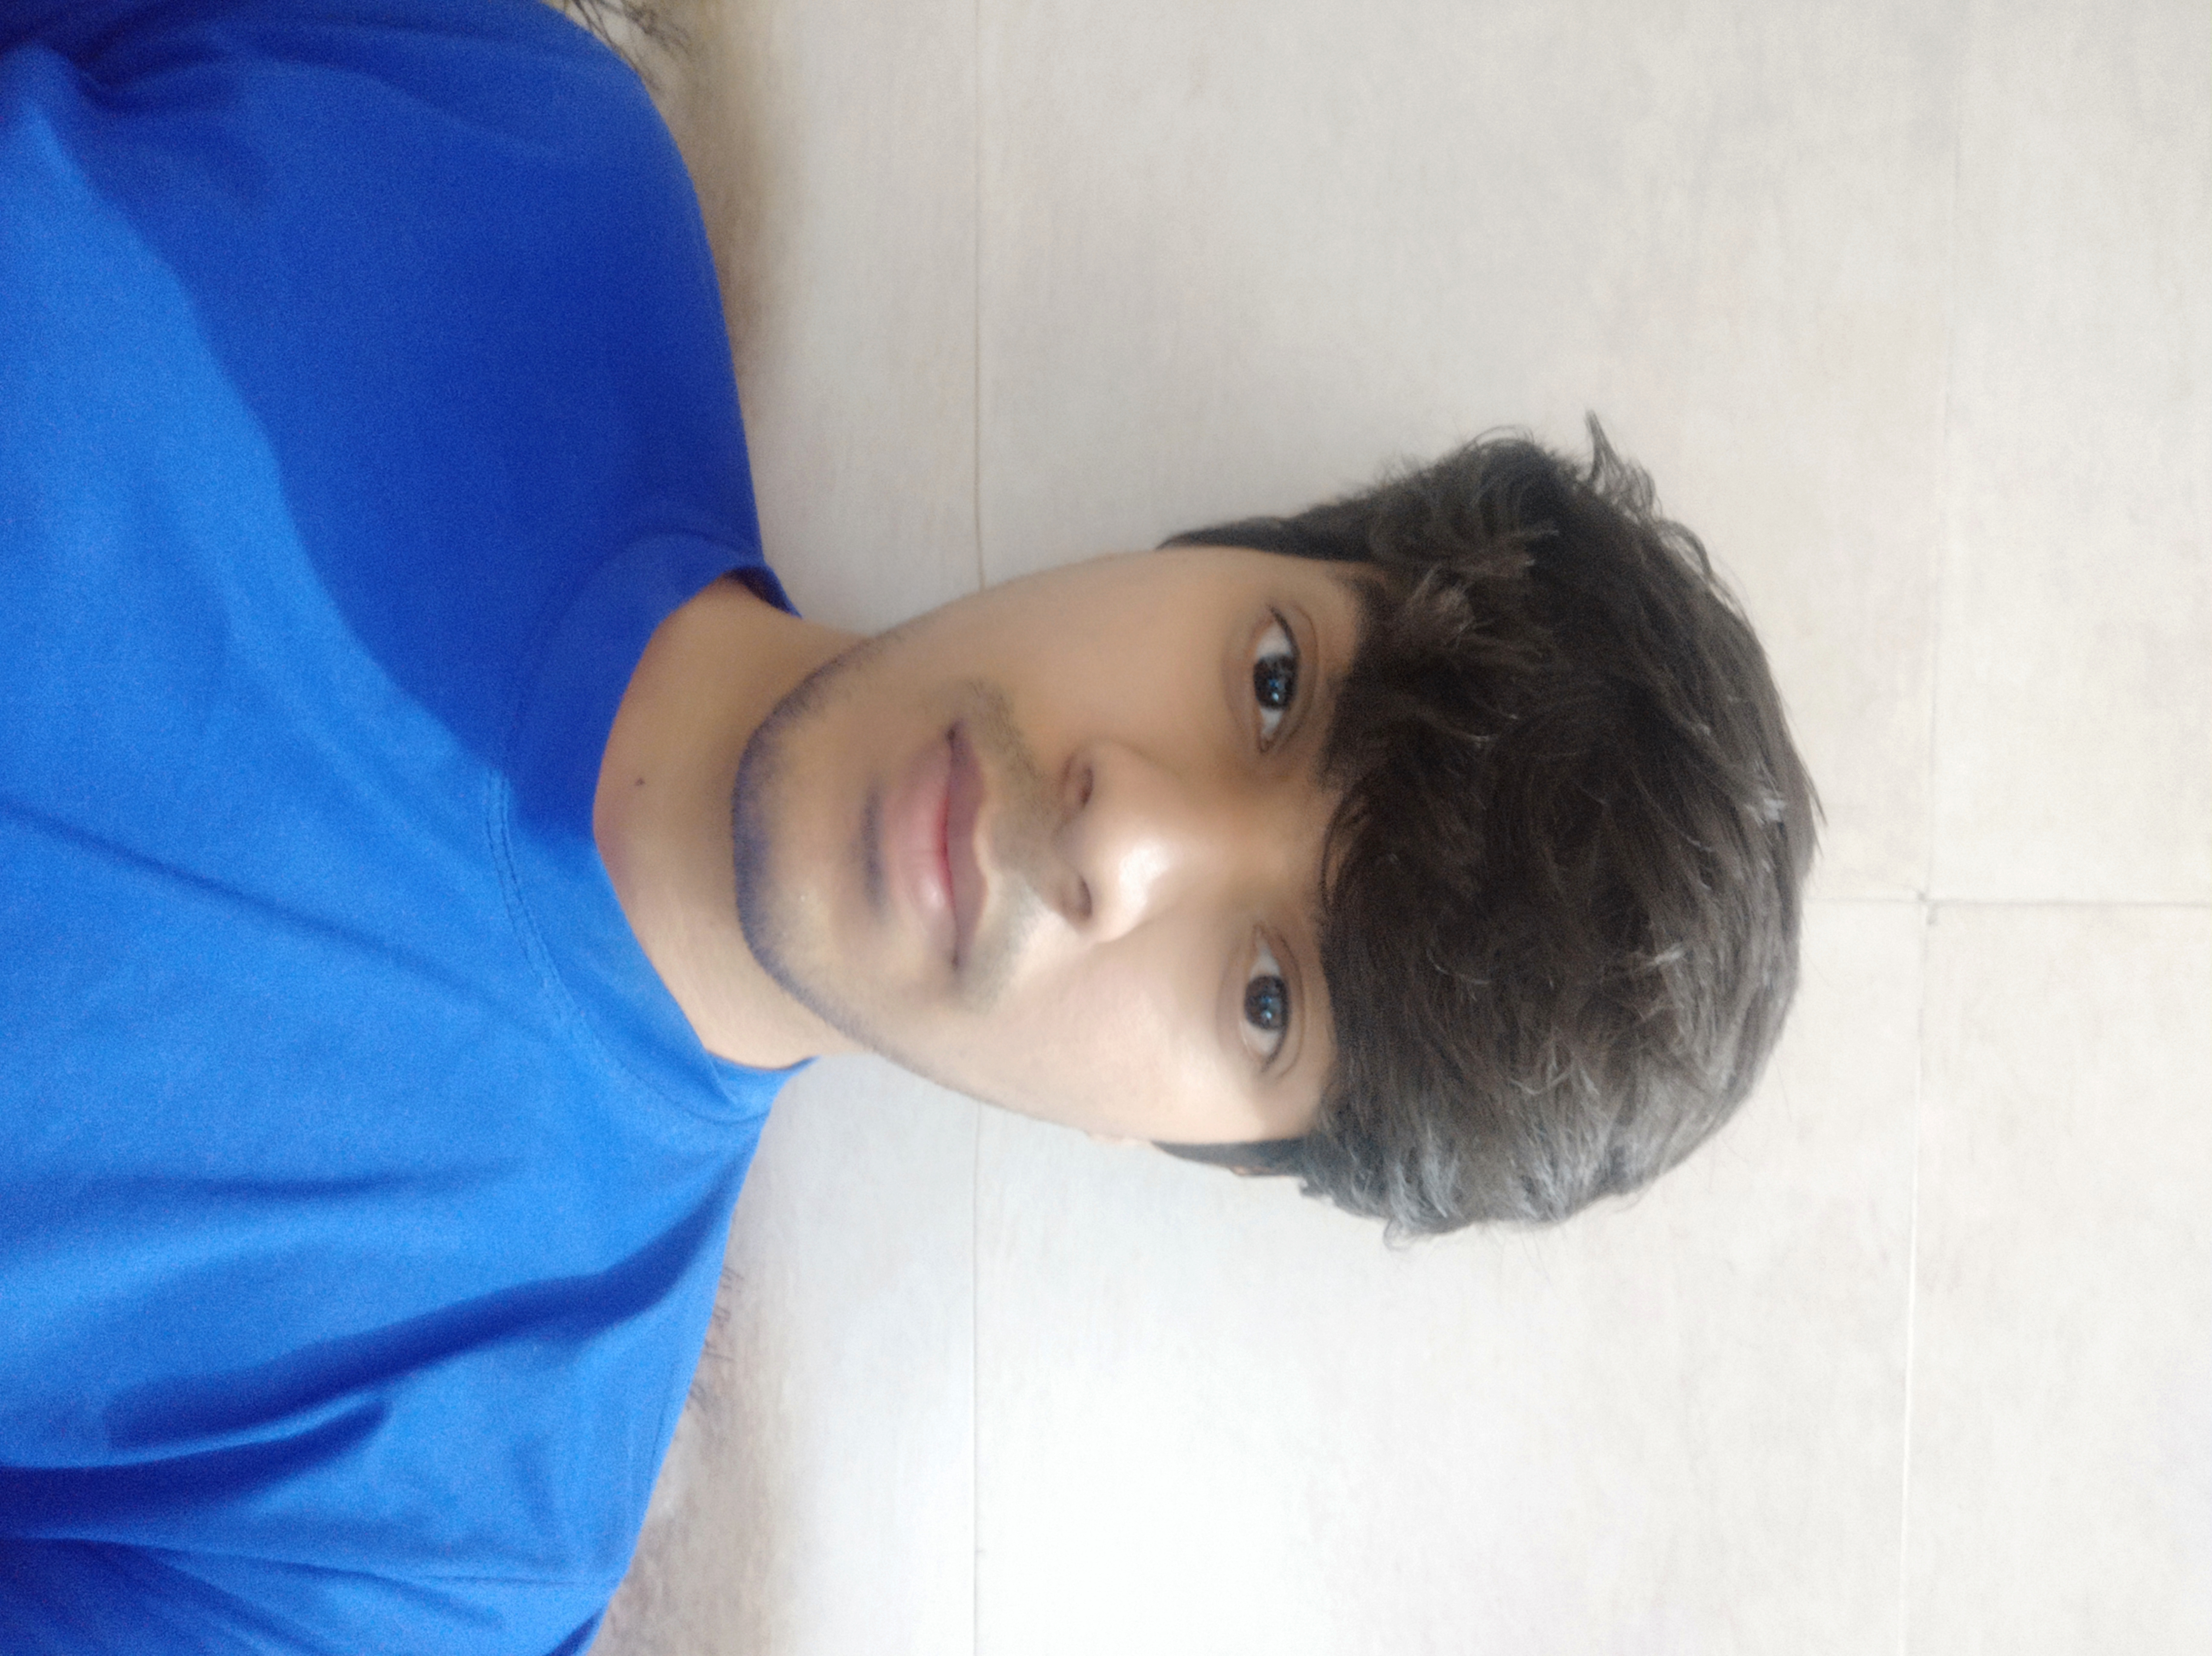
\includegraphics[scale=0.02, origin = c]{profile}}\\
         
        %-----------------------------------------------------------  
        B-98, Panchsheel Vihar & \\
        New Delhi - 110017  \\
        \textbf{Email: }tyagi.aadhar@gmail.com \\
        \textbf{Phone: }8800774261\\
%-----end
\end{tabular*}

\begin{resume}
 \section{OBJECTIVE} To explore and learn new technologies and ideas in the field of computer science. Hoping to obtain as much exposure as possible to expand my skill set, improve social skills as well as gain hands on experience. \\

\section{EDUCATION}\begin{tabu} to 1\textwidth { | X[c] | X[c] | X[c] | X[c]| X[c]|}
 \hline
 Degree & College /School & University & Passing Year & Pass Percentage\\
 \hline
 B. Tech (Software Engineering) & Delhi Technological University &Delhi Technological University & 2021 & 8 (Till Sem 3) \\
\hline
HSC & Apeejay, Sheikh Sarai & CBSE & 2016 & 93.1\\
\hline
SSC & Apeejay, Sheikh Sarai & CBSE & 2014 & 10 GPA\\
\hline
\end{tabu}

\section{PROJECTS } \begin{enumerate}
  \item  {\large{\sl Autonomous Underwater Vehicle}}\\
 Worked to develop control algorithms for the AUV. Implelmented computer vision modules for object detection, obstacle avoidance, path following. Also developed a smart AI to perform the given tasks effieciently as well as make sure the safety of the AUV.\\
        - The   \textbf{control stack} was built on ROS (Robot Operating System). The PIDs were implemented for Roll, Yaw and Pitch axes. Ziegler Nichols method was used to tune the PIDs. Integrated various AHRS (Attitude Heading and Reference System) and INS + GPS (Inertial Navigation System) such as VectorNav 300 and Xsens MTI series using ROS nodes. Developed a network like structure using ActionLib for efficient transfer of data and decision making.\\
        - The   \textbf{vision stack} was built mainly on OpenCV, underwater image enancement techniques from several research papers were implemented and tested, computer vision algorithms for detection, trained custom YOLO on Darknet.\\
	- Implemented   \textbf{decision making} through state machines (SMACH), python API, integrated with ROS ActionLib. Also worked on microcontrollers (Arduino, Atmega) and their interfacing and communication with SBC.
 \item {\large{\sl Eyantra, 2018, Pollinator Bee}}\\
 Worked on developing a Autonomous drone capable of waypoint navigation using whycon coordinates provided from the camera overhead.\\
  	- Implemented PIDs for Roll and Pitch for a drone on ROS python. Learned drone mechanics, whycon coordinates, simulated the drone in V-REP. \\
	- Developed robust OpenCV algorithms for detection of LEDs. \\
\\
 \item {\large{\sl Others}}\\

  	- Haar Cascade based stone paper scissor game. \\
	- Compter Vision, gesture password unlocker. Unlock your computer using your hand gestures and webcam.\\
	- .\textbf{Few Shot Learning}, character  classifier, siamise network,  Omniglot dataset. \\
	- ANN, python implementation of levenberg marquardt algorithm.\\
	- \textbf{Visual Odometry} and VISP based path tracing in Turtlebot, Gazebo.\\
	\end{enumerate}


\end{resume}
\end{document}